\section{Key experiments that established quantum mechanics (8/26)}

\referto{\weinberg~Chap 1. For further reading, try \anastopolous~Chap 2, \shankar~3.}

Quantum mechanics was first motivated by a series of experiments that cannot be explained by classical mechanics and statistical physics. These exceptions to classical physics happen in the microscopic world, when the scale of physical quantities, such as energy, angular momentum and electric charge becomes comparable to certain characteristic scales.

The quantization of energy was observed in both light and atomic spectra, which motivated Planck, Einstein and others to propose a discretized (``quantized'') energy levels for photons and atoms. Bohr was able to explain the Rydberg formula\cite{Rydberg1890} of hydrogren atom spectral lines under the assumption of a quantized angular momentum for electrons, which was later observed in the Stern-Gerlach experiment\cite{Gerlach1922}. After de Broglie first proposed the wave nature of microscopic particles such as electrons, Davisson and Germer\cite{Davisson1927} were able to directly observe it in the diffraction pattern of electrons scattered by a nickel crystal. These experiments call for a new theory framework that defeats the intuition of classical physics. 

\subsection{Energy quantization of light in terms of photons}

Young's double-slit experiment clearly demonstrated the wave nature of light, whose energy should change continuously in classical electromagnetism. However, this point of view is seriously challenged by black-body radiation. 

\subsubsection{Black-body radiation and Planck's formula} 

Consider light in a cubic box (a simplified model of a black body) of volume $L^3$. A standing wave in the box satisfies the following condition for its wavevector $\vec k=(k_x,k_y,k_z)$:
\begin{align}
  \lambda_i=\frac{2\pi}{k_i}=\frac{2L}{n_i},~~~n_i=1,2,3,\cdots,~~~i=x,y,z  
\end{align}
Counting the number of standing wave modes in the box in terms of frequency $\nu=ck/2\pi$
\begin{align}
\int\text{d}k_x\text{d}k_y\text{d}k_z=\frac184\pi\int k^2\text{d}k=(\frac{\pi}{L})^3\sum_{\{n_i\}}=(\frac{\pi}{L})^3N_\text{modes}
\end{align}
we have the density of states for light-wave modes per unit volume:
\begin{align}
\frac{1}{L^3}\frac{\text{d}N}{\text{d}\nu}=(\frac{1}{\pi})^3\frac\pi2 k^2\frac{\dif k}{\dif\nu}=\frac{8\pi}{c^3}\nu^2
\end{align}
Assuming the equipartition theorem in classical physics, i.e. each mode carries an averaged energy of $k_BT$, the black-body radiation energy per unit volume is
\begin{align}
\frac{\dif E}{L^3\dif\nu}=\frac{k_BT}{L^3}\frac{\text{d}N}{\text{d}\nu}=\frac{8\pi k_BT}{c^3}\nu^2
\end{align}
This is known as the Rayleigh-Jeans formula and it correctly captures the long-wavelength (small $\nu$) behavior of universal black-body radiation, first established by Kirchhoff around 1860. However, it diverges in the short wavelength limit, known as the ultraviolet catastrophe. Experimentally the Wien's Distribution Law was observed at short wavelengths:
\begin{align}
\frac{\text{d}E}{L^3\text{d}\nu}\sim\nu^3e^{-\alpha(T)\nu}
\end{align}
In order to reconcile long-wavelength Rayleigh-Jeans formula to short-wavelength Wien's law, Planck came up with his famous formula:
\begin{align}\label{planck formula}
\frac{\text{d}E}{L^3\text{d}\nu}=\frac{8\pi\nu^2}{c^3}\frac{h\nu}{e^{\alpha\nu}-1},~~~\alpha=\frac{h}{k_BT}
\end{align}
where the Planck constant is 
\begin{align}
h=6.63\times10^{-34}~J\cdot s
\end{align}
Planck's formula (\ref{planck formula}) indicates that the statistical-averaged energy of light at frequency $\nu$ is given by
\begin{align}
U(\nu)=\frac{h\nu}{e^{h\nu/K_BT}-1}=\frac{\sum_{n\in\mbz_+}nh\nu e^{-nh\nu/K_BT}}{\sum_{n\in\mbz_+}e^{-nh\nu/k_BT}}
\end{align}
under Planck's quantization hypothesis that the microscopic states of light have energy $nh\nu$ where $n\in\mbz_+$ is a positive integer. 

\subsubsection{Einstein's ``light quantum'' and photoelectric effect}

Motivated by Planck's quantization hypothesis, based on the assumption that light gives out energy in multiples of energy quantum $h\nu$, Einstein predicted the photoelectric effect
\begin{align}
K_{\text{max}}=eV=h\nu-\Phi
\end{align}
where $K_{max}$ is the maximal kinetic energy of emitted photoelectrons when light of frequency $\nu$ shines on a metal, and $\Phi$ is the work function of the metal. $V$ is minimal voltage that is required to stop photoelectron emission. This experiment was carried out by Millikan\cite{Millikan1916}, who obtained Planck's constant
\begin{align}
h=e\frac{\dif V}{\dif\nu}
\end{align}


\subsubsection{Compton effect demonstrated quantization of light in terms of photons}

\begin{figure}
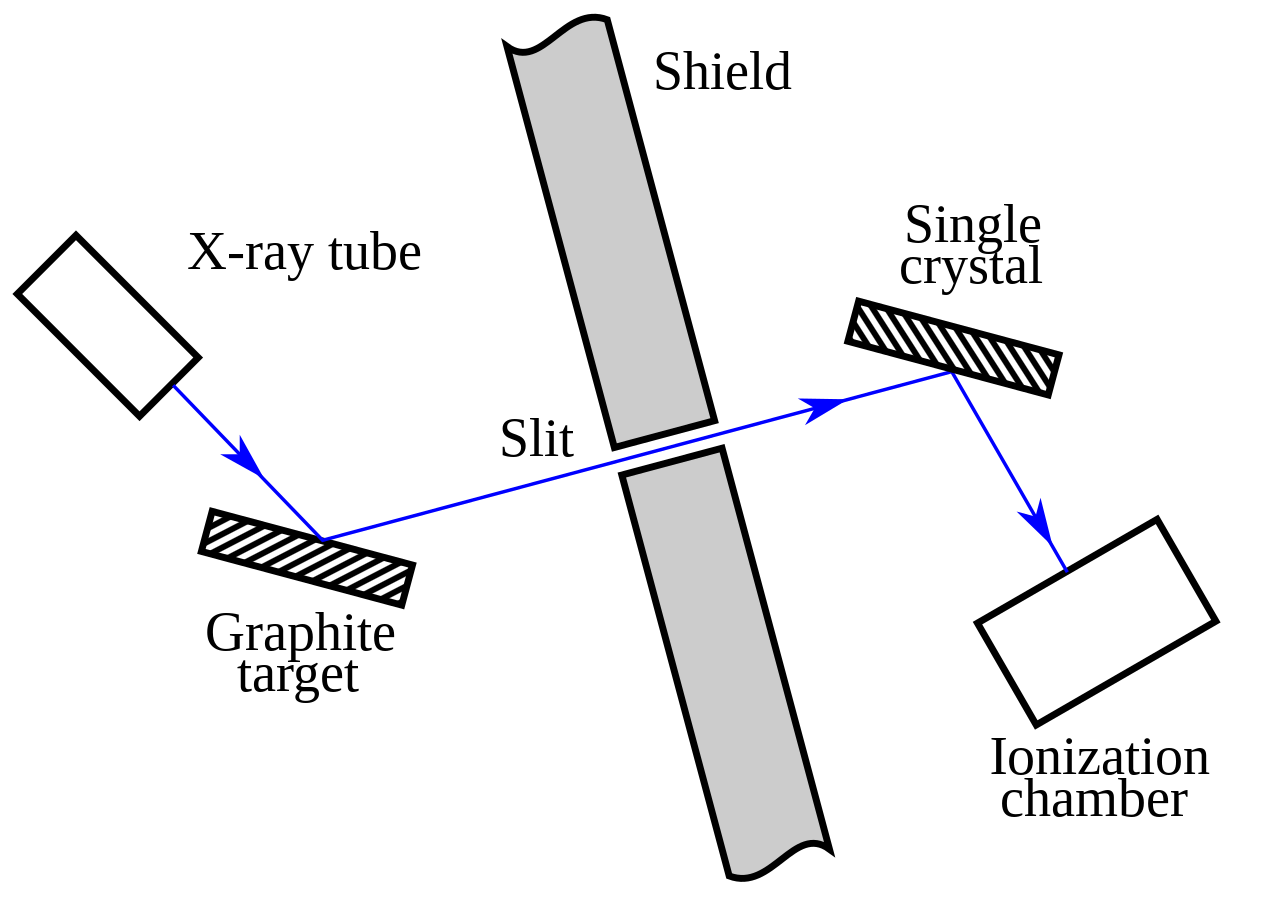
\includegraphics[width=0.45\columnwidth,alt={Schematic setup of Compton's experiment.}]{figures/compton1.png}%
\;~~~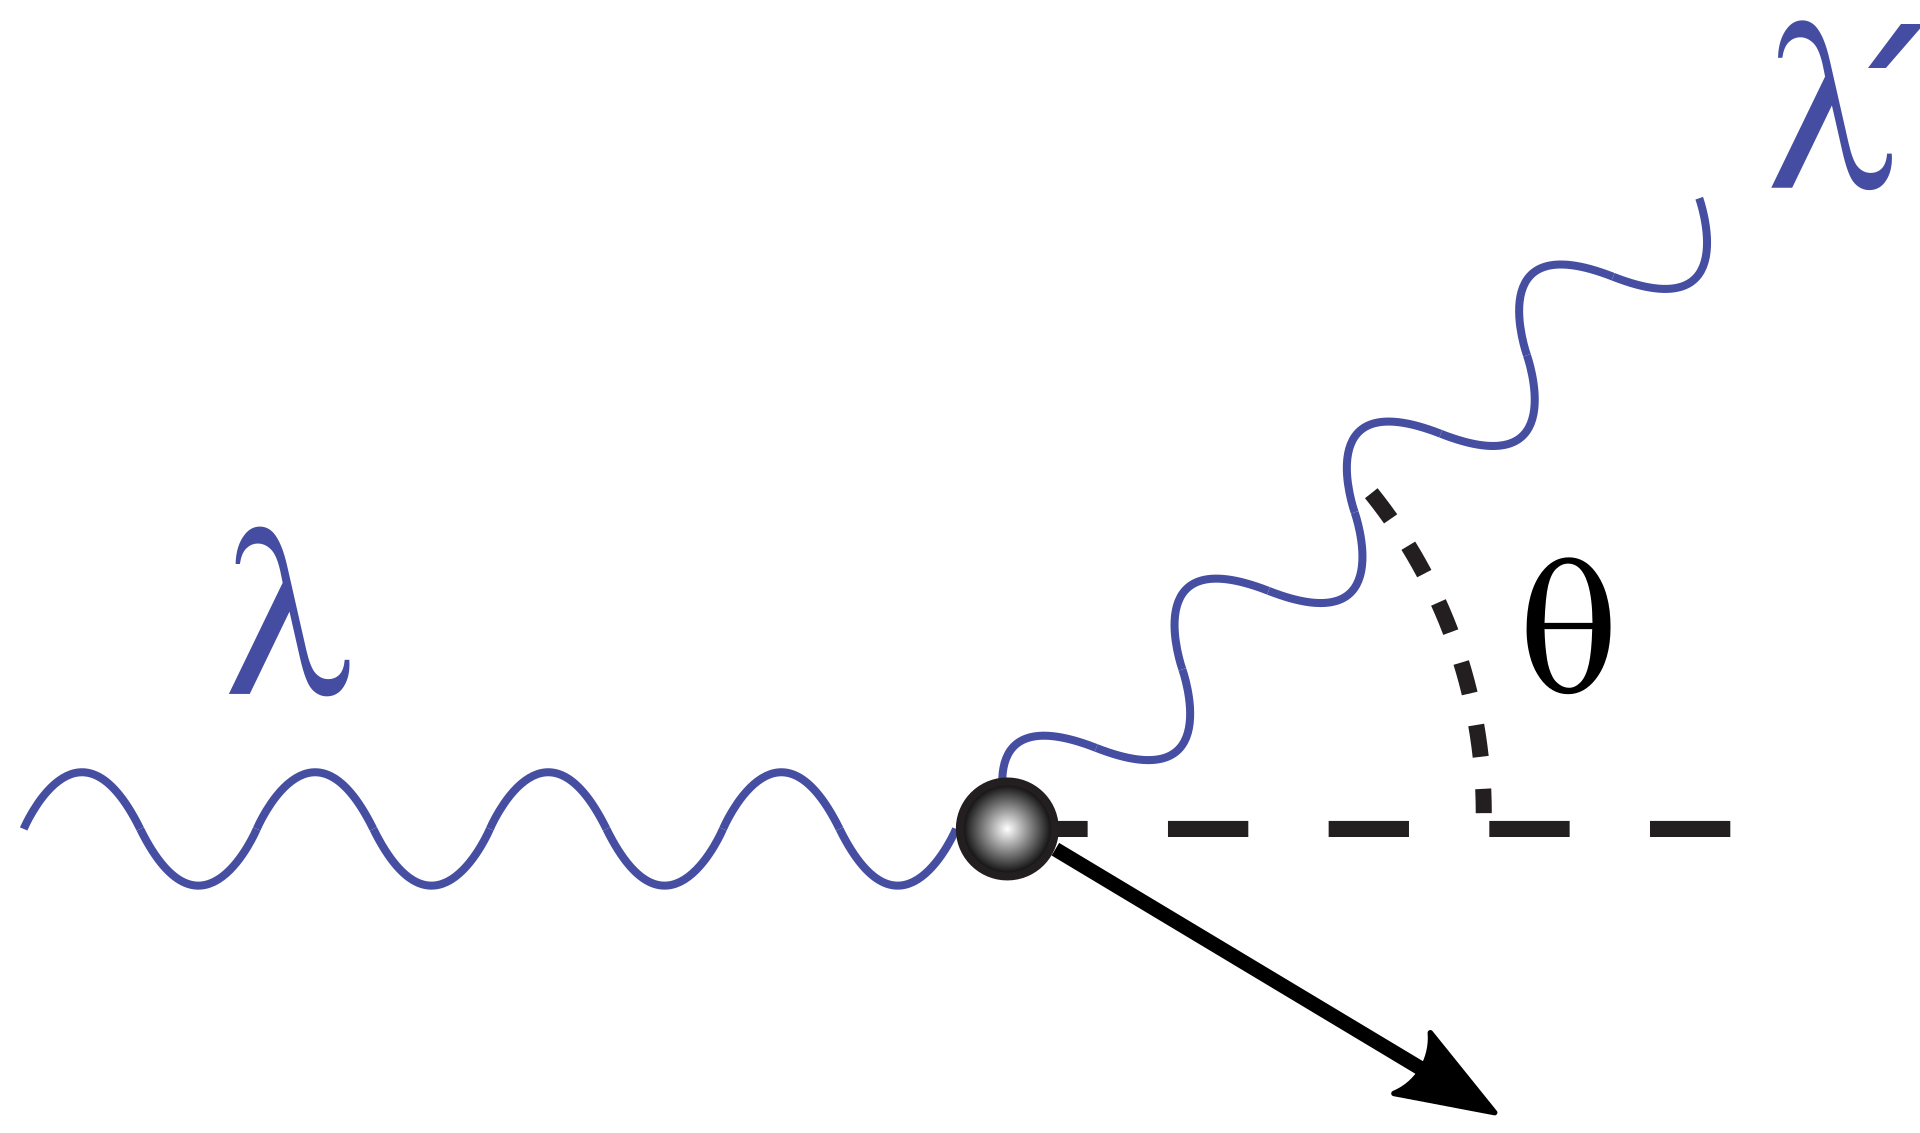
\includegraphics[width=0.45\columnwidth,alt={Photon–electron scattering diagram used to explain the Compton effect.}]{figures/compton2.png}
\caption{(Left) Schematic setup of Compton's experiment. (Right) The light-electron scattering process in the Compton experiment.}
\label{fig:compton}
\end{figure}

Discovered by Arthur Compton in 1923\cite{Compton1923}, when the energy of the X ray photon ($\sim$17 keV) was significantly larger than the binding energy of the atomic electron, the electrons could be treated as being free after scattering. In this case, a \emph{Compton shift} between the wavelengths of injected light ($\lambda$) and the scattered light ($\lambda^\prime$) was observed to satisfy the following relation with the scattering angle $\theta$ (see Fig. \ref{fig:compton}):
\begin{align}
\lambda^\prime-\lambda=\frac{h}{m_ec}(1-\cos\theta)
\end{align}
where $h$ is the Planck's constant.

The Compton shift can be explained by energy and momentum conservation, by assuming the photon energy of $E=h\nu=hc/\lambda$. 


\subsection{Quantization of atomic energy levels}


\subsubsection{Rydberg formula for the spectral lines in a hydrogen atom}

After the discovery of dark lines in the spectrum of the sun at the beginning of 18th century, it was later realized that hot atomic gases absorb and emit light only at certain definite frequencies. Building on works of Balmer and others, Rydberg discovered the following rule\cite{Rydberg1890} for the frequency of emitted light from hydrogen gases:
\begin{align}\label{rydberg rule}
\nu=\frac c\lambda=cR_H(\frac1{n^2}-\frac1{m^2}),~~~m,n\in\mbz_+.
\end{align}
This clearly demonstrated the discreteness of atomic energy levels $E_n\propto\frac1{n^2}$, further motivating Bohr's theory of the hydrogen atom. 

\subsubsection{Franck-Hertz experiment}

In the Franck-Hertz experiment (1914) illustrated in Fig. \ref{fig:franck-hertz}, in a vacuum tube fitted with three electrodes (an electron-emitting, hot cathode; a metal mesh grid; and an anode), when a grid voltage is applied between the cathode and the anode, the electric current through the tube filled with thin mecury vapours, due to electrons that pass through the grid and reach the anode, is measured in the experiment. As shown in the middle figure, the current increases rapidly at low voltages, and then sharply drops almost back to zero at 4.9 V, with similar effects observed as 9.8 V and other multiples of 4.9 V. This can be understood by the quantized energy levels of mercury atoms. inside the single mercury droplet in the vacuum tube, as shown in Fig. \ref{fig:franck-hertz}.

\begin{figure}
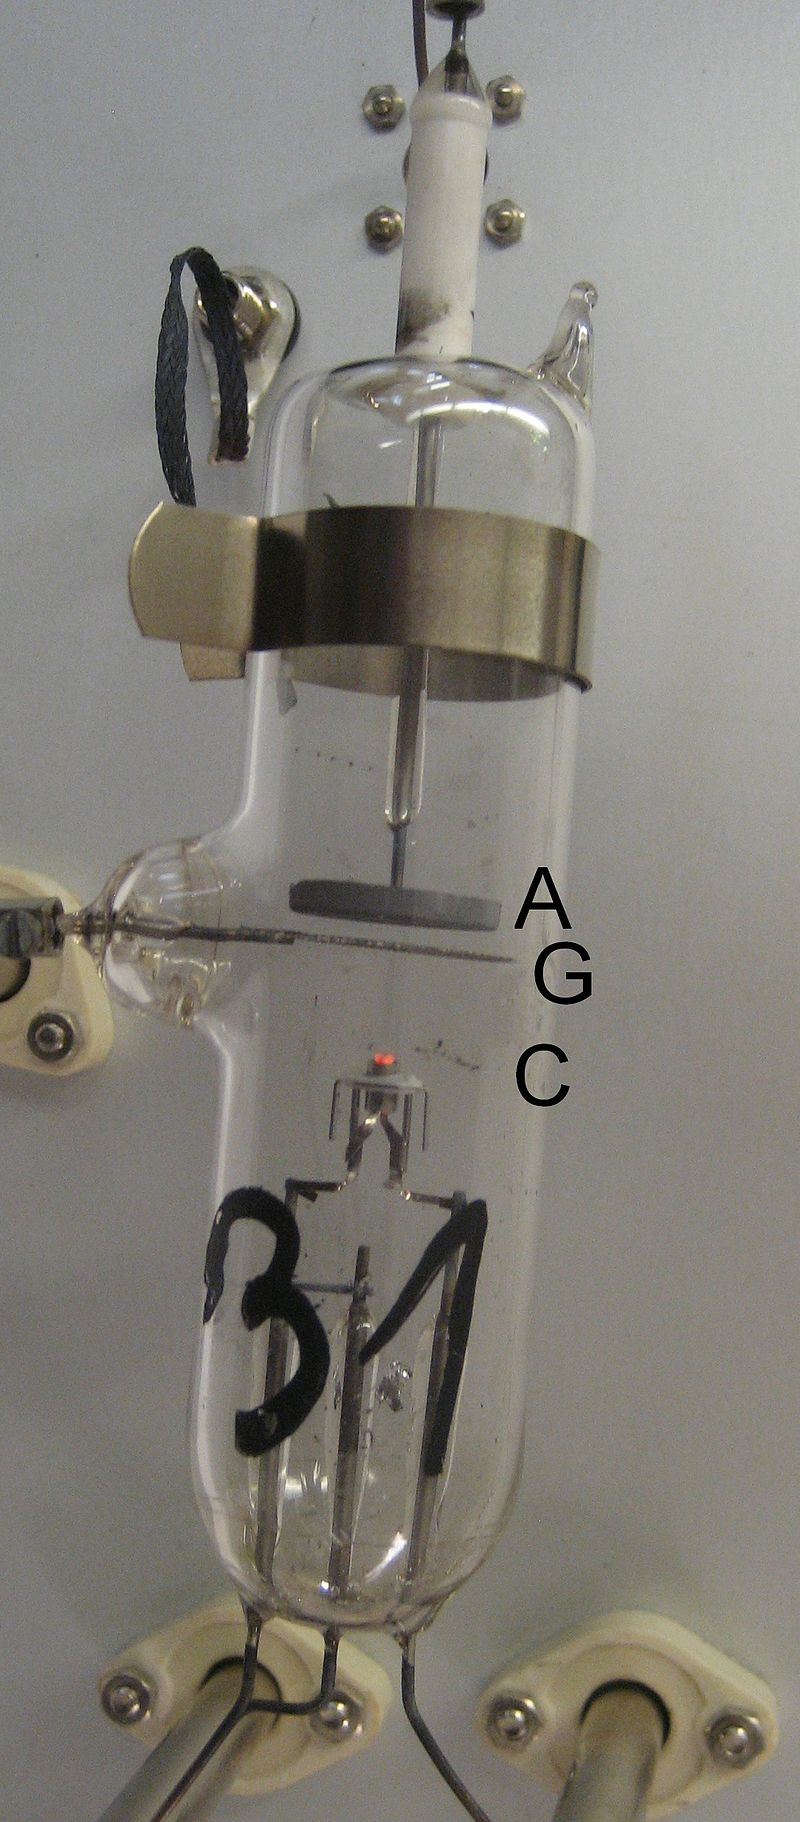
\includegraphics[width=0.2\columnwidth,alt={Photo of a vacuum tube used for the Franck–Hertz experiment.}]{figures/fh1.jpg}%
\;~~~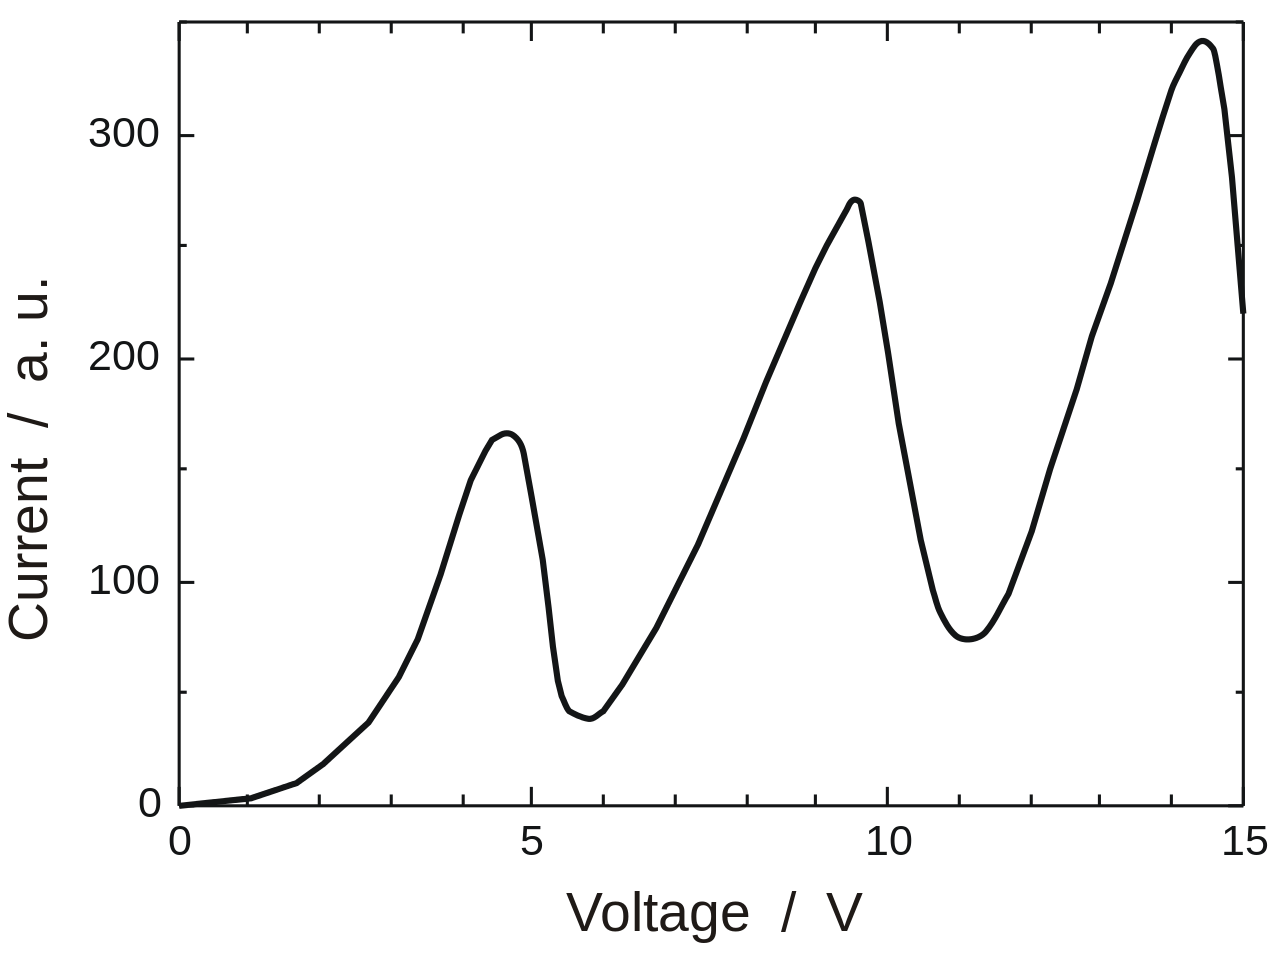
\includegraphics[width=0.45\columnwidth,alt={Anode current versus grid voltage showing peaks and drops at multiples of about 4.9 V.}]{figures/fh2.png}%
\;~~~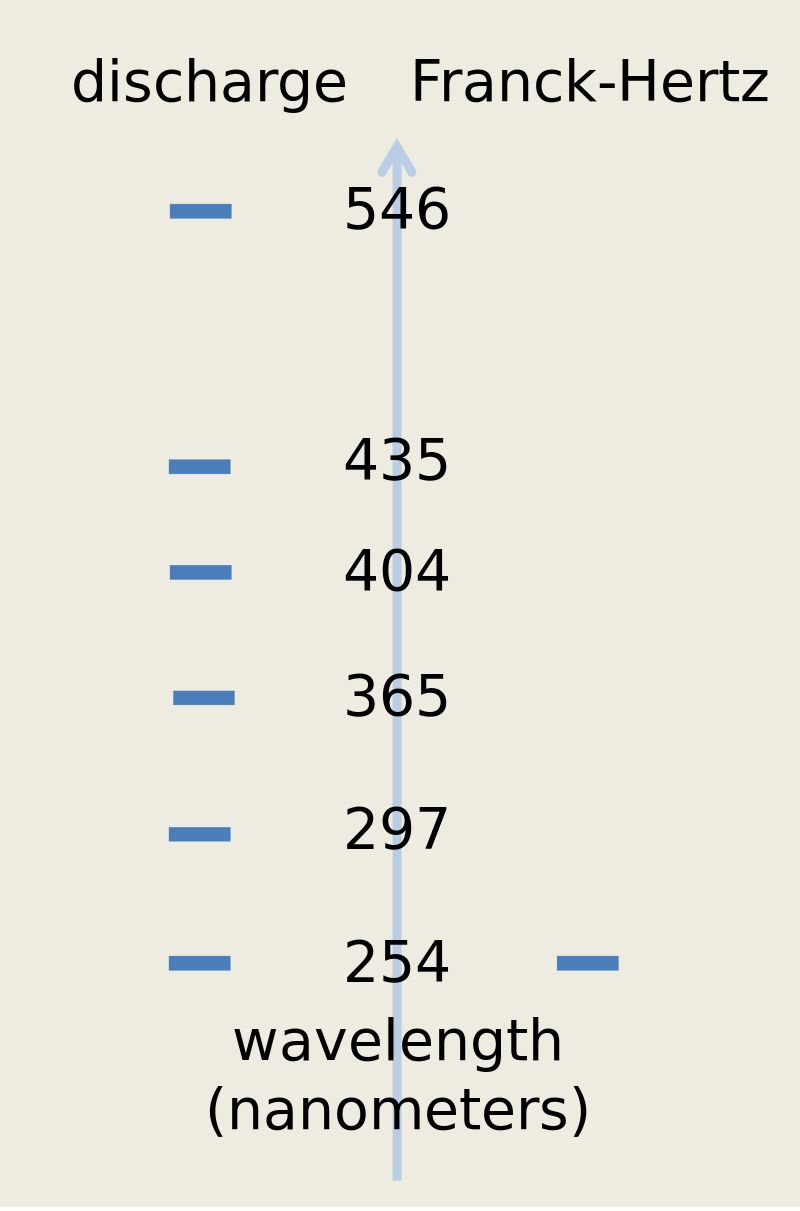
\includegraphics[width=0.25\columnwidth,alt={Mercury emission spectrum comparison for a discharge tube and a Franck–Hertz tube in operation.}]{figures/fh3.png}
\caption{(Left) Photograph of a vacuum tube used for the Franck-Hertz experiment. (Middle) Anode current (arbitrary units) versus the grid voltage relative to the cathode. (Right) Wavelengths of light emitted by a mercury vapor discharge and by a Franck-Hertz tube in operation at 10 V. (Picture from Wikipedia)}
\label{fig:franck-hertz}
\end{figure}



\subsection{Quantization of angular momentum}


\subsubsection{Bohr's explanation of hydrogen atom spectral lines}

Rydberg's rule\cite{Rydberg1890} indicates that the photon energy emitted by the hydrogen atom is given by
\begin{align}
h\nu=E_m-E_n,~~~E_n=-\frac{hcR_H}{n^2},~n\in\mbz_+.
\end{align}
How to explain the $1/n^2$ quantization of hydrogen atom energy levels? According to classical mechanics, for an electron in the Coulomb force field of hydrogen nucleus, its speed $v$ and radius $r$ satisfies
\begin{align}
\frac{mv^2}{r}=\frac{ke^2}{r^2}\Longrightarrow E=\frac12mv^2-\frac{ke^2}r=-\frac{ke^2}{2r}
\end{align}
where $k$ is the Coulomb constant. To fit the $n^2$ dependence of the orbit radius $r$, Niels Bohr came up with the following quantization condition for angular momentum:
\begin{align}
mvr=n\hbar
\end{align}
where $\hbar$ turns out to be $h/2\pi$. This quantization condition leads to the famous energy levels of electrons in a hydrogen atom:
\begin{align}
E_n=-\frac{mk^2e^4}{2\hbar^2}\frac1{n^2}=-\frac{13.6~\text{eV}}{n^2}
\end{align}

\subsubsection{Stern-Gerlach experiment demonstrated the quantization of angular momentum}

\begin{figure}
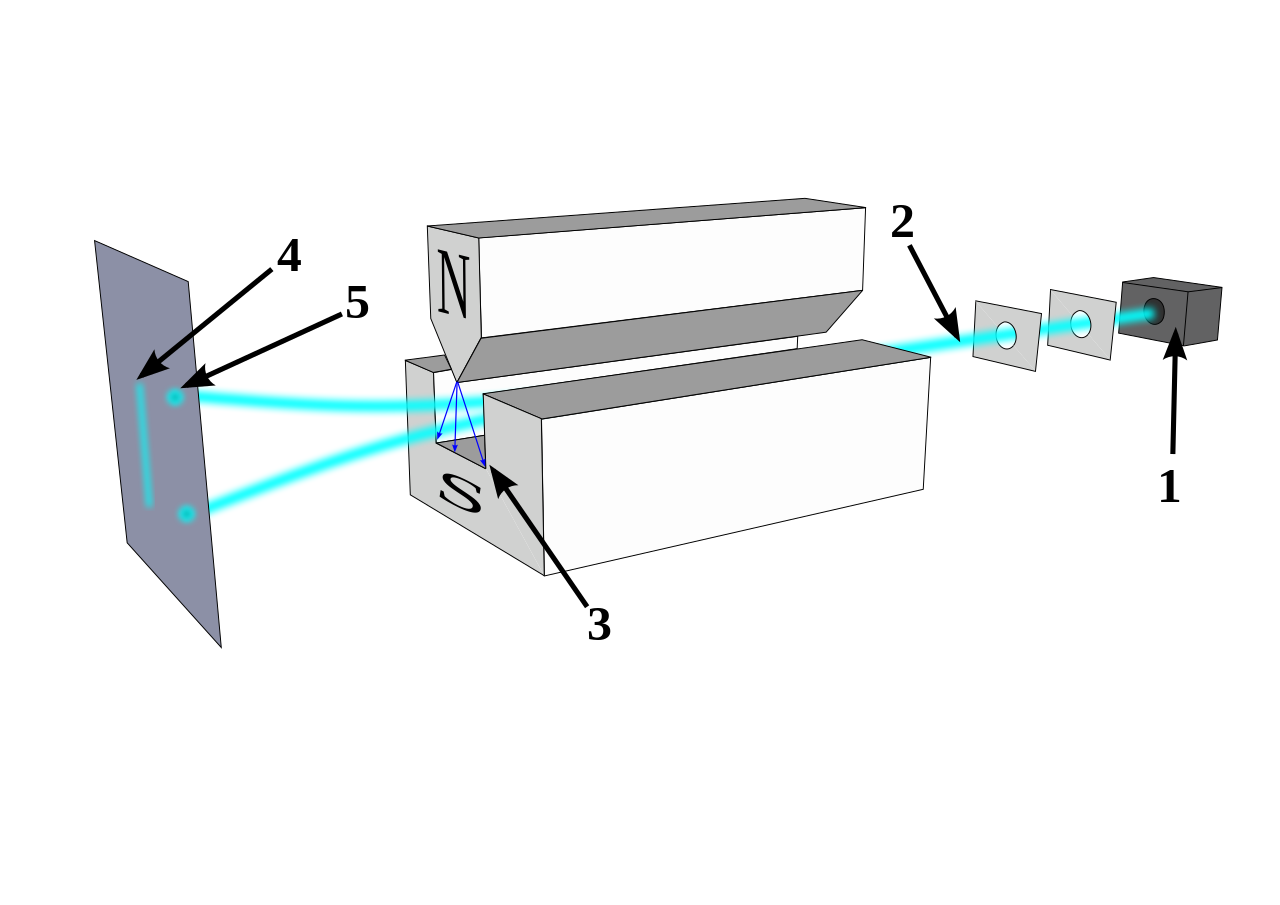
\includegraphics[width=0.8\columnwidth,alt={Stern–Gerlach apparatus showing a silver-atom beam split into two components in an inhomogeneous magnetic field.}]{figures/sg1.png}
\caption{Schematic setup of Stern-Gerlach experiment: Silver atoms travelling through an inhomogeneous magnetic field, being deflected up or down depending on their spin. (1) furnace, (2) beam of silver atoms, (3) inhomogeneous magnetic field, (4) the classically expected result, (5) the observed result.}
\label{fig:stern gerlach}
\end{figure}

In 1922 Stern and Gerlach performed an experiment\cite{Gerlach1922} measuring the deflection of silver atoms by an inhomogeneous magnetic field, as illustrated in Fig. \ref{fig:stern gerlach}. Due to the interaction energy $U=-\vec\mu\cdot\vec B$ of a magnetic moment $\vec\mu$ under a magnetic field $\vec B=B_z\hat z$, a non-uniform magnetic field exerts a force $\vec F=-\vec\nabla U=\mu_z\vec\nabla B_z$ on the moment-carrying silver atoms, therefore deflecting the silver atom beams in the inhomogenous magnetic field. As shown in Fig. \ref{fig:stern gerlach}, in contrast a continuous range of values of the magnetic moment as expected in classical mechanics, the experimental observations pointed to quantization of magnetic moment $\mu_z=g\mu_BS_z/\hbar$, where we defined $\mu_B$ as the Bohr magneton:
\begin{align}\label{Bohr  
   magneton}
\mu_B=\frac{\hbar e}{2m_e}
\end{align}
$g\approx 2$ as the electron $g$-factor and
\begin{align}
S_z=\pm\frac\hbar2
\end{align}
is the quantized spin angular momentum of a silver atom observed in Stern-Gerlach experiment.

This experiment demonstrated that in addition to energy level quantization, other physical observable such as spin angular momentum are also quantized in microscopic scales such as in silver atoms. Moreover, we can consider sequential Stern-Gerlach experiments shown in Fig. \ref{fig:stern gerlach sequentials}, where silver atoms are deflected by multiple inhomogeneous magnetic fields in a sequence. Remarkably, unlike the classical case of light passing through polarizers, which filter out everything after two polarizers with perpendicular polarization axes, two quantum mechanical ``beam splitters'' with perpendicular magnetic field directions still allows two splitted beams to pass through, as illustrated in the middle and bottom parts of Fig. \ref{fig:stern gerlach sequentials}.

\begin{figure}
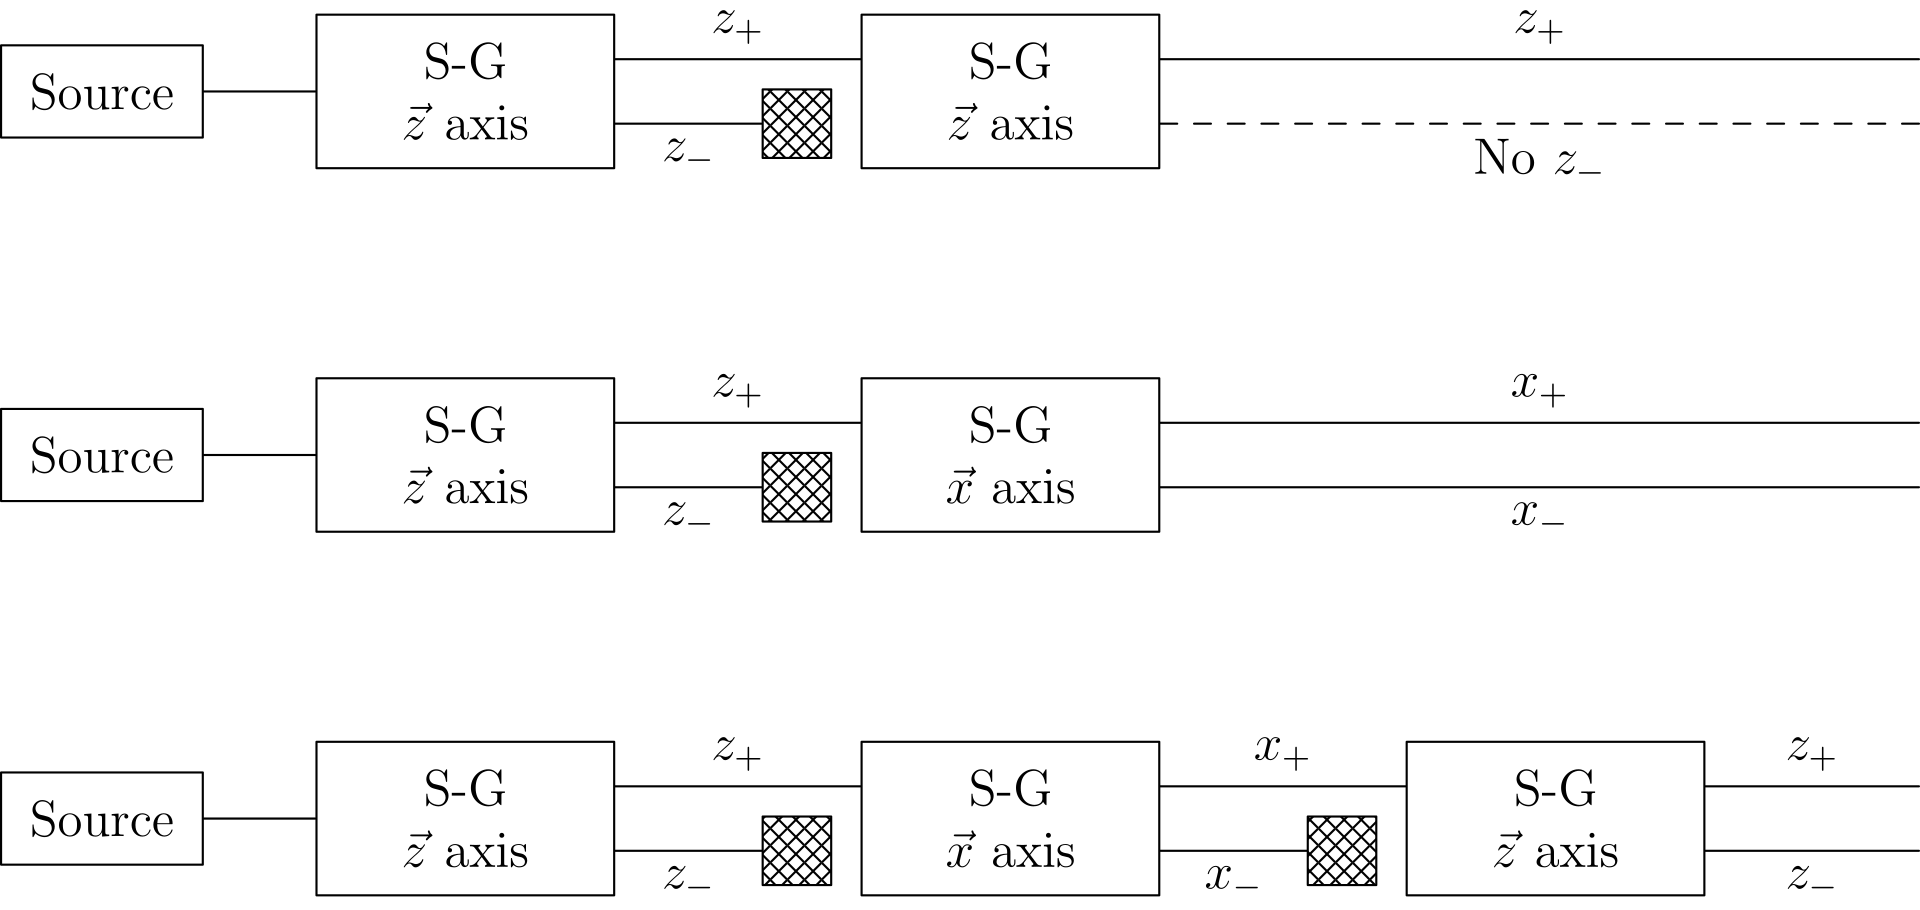
\includegraphics[width=0.9\columnwidth,alt={Sequential Stern–Gerlach setups illustrating outcomes for different magnetic-field orientations.}]{figures/sg2.png}
\caption{Sequential Stern-Gerlach experiments. (Picture from \sakurai)}
\label{fig:stern gerlach sequentials}
\end{figure}

\subsection{Davisson-Germer experiment demonstrated the wave nature of electrons}

In 1924 de Broglie formally proposed the wave nature of electrons and other particles, in terms of their de Broglie wavelengths:
\begin{align}\label{de Broglie wavelength}
\lambda=\frac{h}{p}
\end{align}
where $p$ is the momentum of the particle. If this proposal were true, it means that microscopic particles such as electrons should exhibit interference phenomena in the same way as acoustic and light waves. 

\begin{figure}
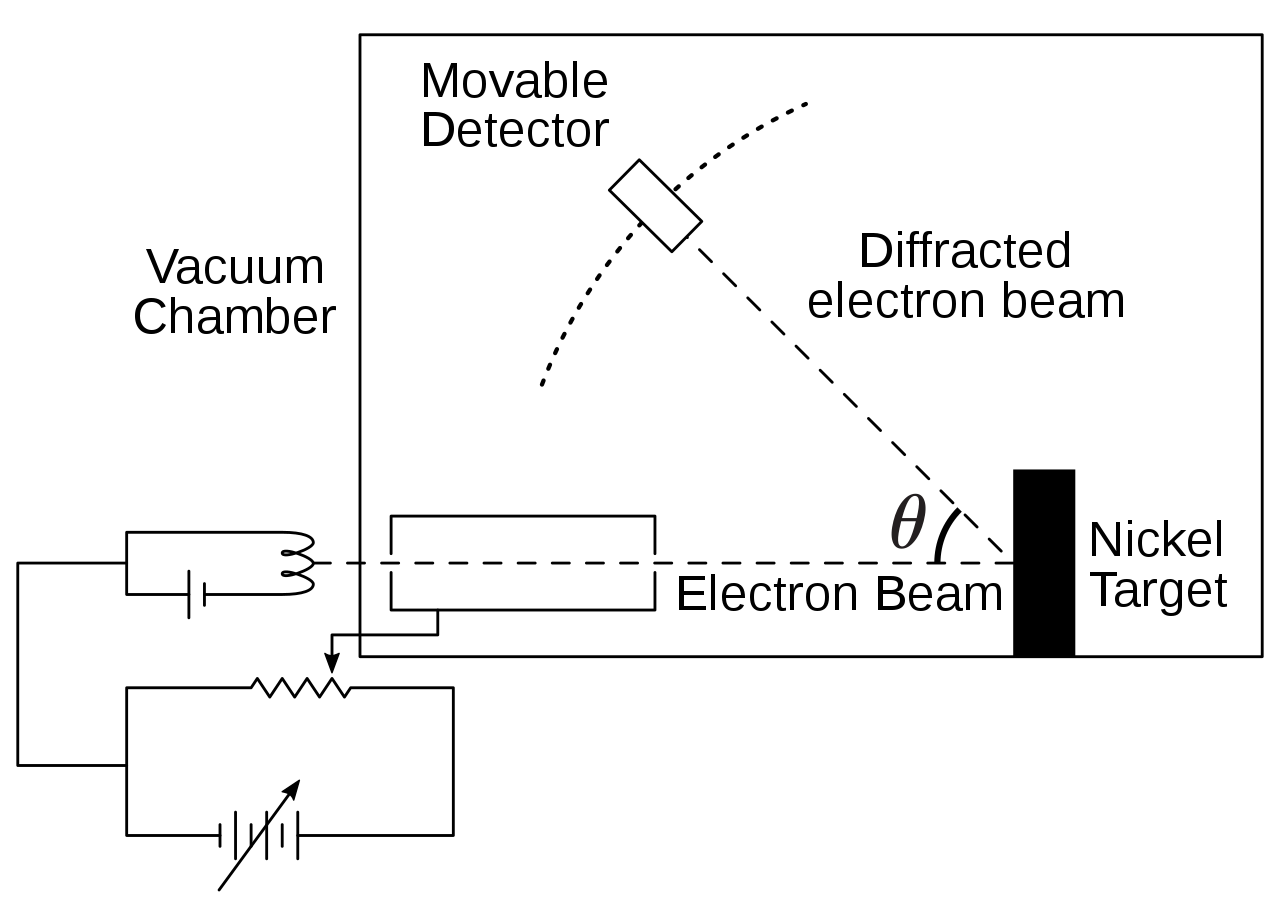
\includegraphics[width=0.45\columnwidth,alt={Davisson–Germer experimental setup schematic for electron diffraction from a crystal.}]{figures/dg1.png}%
\;~~~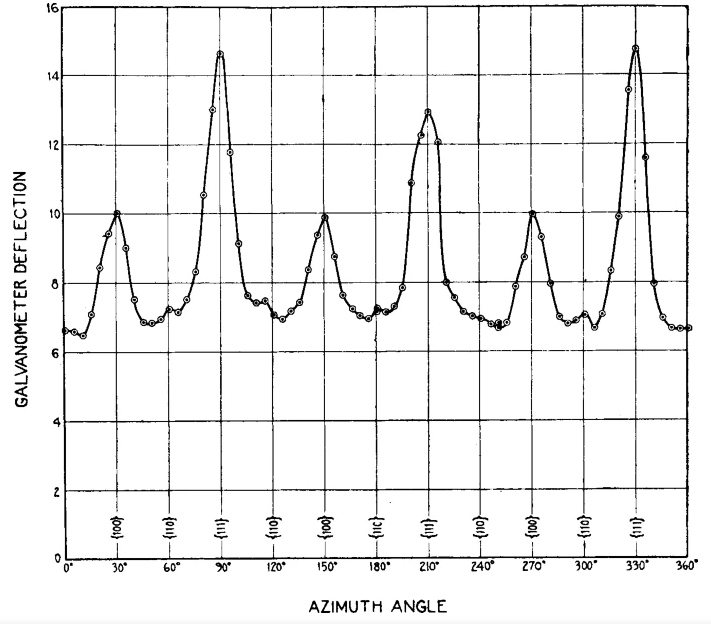
\includegraphics[width=0.4\columnwidth,alt={Plot of electron scattering intensity versus angle showing a diffraction peak at a given voltage.}]{figures/dg2.png}
\caption{(Left) Schematic setup of Davisson-Germer experiment. (Right) Intensity of electron scattering vs. azimuth angle at 54 volts, co-latitude $\theta=50^o$.}
\label{fig:davisson germer}
\end{figure}

In 1927 Davisson and Germer\cite{Davisson1927} performed an experiment to observe the diffraction pattern of electrons scattered by the surface of a crystal of nickel metal, as shown in Fig. \ref{fig:davisson germer}. The highest intensity was observed at an angle $\theta=50^o$ with a voltage of 54 V, giving the electrons a kinetic energy of 54 eV. To be compatible with the Bragg's law
\begin{align}\label{brag's law}
n\lambda=2d\sin(90^o-\theta/2),~~~n\in\mbz_+.
\end{align}
with the lattice spacing of nickel $d=0.091$ nm, the $n=1$ Bragg peak in (\ref{brag's law}) exactly corresponds to the de Broglie wavelength (\ref{de Broglie wavelength}) of electrons. We will examine the experimental results in Fig. \ref{fig:davisson germer} more carefully in Homework 1.